\chapter{Resultados Parciais}
\label{cap:04}

\newcommand{\capturaoupendente}[2]{%
	\IfFileExists{#1}{\includegraphics[width=\textwidth]{#1}}{%
		\fbox{\parbox{0.9\textwidth}{\centering\vspace{1.2cm}\textbf{[Inserir captura de tela: #2]}\par\texttt{#1}\vspace{1.2cm}}}}}

Os resultados parciais correspondem às etapas do diagrama da Figura~\ref{fig:metodologia} concluídas até a qualificação. O núcleo bioinformático (\ref{oe:dados} a \ref{oe:modulo}) foi implementado e executado para três genes e quatro proteomas, a demonstração gráfica da interface foi produzida (\ref{oe:software}) e a validação (\ref{oe:validacao}) foi realizada em parte. A API e a interface web ainda não foram desenvolvidas. Os resultados comparam sequências de proteínas e não permitem inferir diferenças de sabor, pois o sabor é um traço multifatorial (Seção~\ref{sec:cafe}).

\section{Dados Utilizados e Qualidade dos Proteomas}

Esta etapa correspondeu ao \ref{oe:dados}. Os arquivos multi-FASTA dos proteomas preditos foram obtidos do \textit{Coffee Genome Hub} \cite{Dereeper2015, CoffeeHub}. Entre os seis proteomas disponíveis, foram escolhidos os quatro de melhor qualidade, e os proteomas de ET-39 e de \textit{C. humblotiana} foram descartados por apresentarem montagem fragmentada. Os indicadores dos quatro proteomas selecionados estão na Tabela~\ref{tab:qualidade}.

\FloatBarrier
\begin{table}[!htbp]
	\centering
	\SingleSpacing\small
	\caption{Indicadores de qualidade dos proteomas selecionados}
	\begin{tabularx}{\textwidth}{@{}lYYYY@{}}
		\toprule
		\textbf{Proteoma} & \textbf{Proteínas} & \textbf{Cromossomos} & \textbf{Redundância (\%)} & \textbf{Mediana (aa)} \\
		\midrule
		\textit{C. arabica} Geisha      & 26.367 & 11 & 0,42 & 348 \\
		\textit{C. arabica} Red Bourbon & 33.989 & 11 & 8,52 & 338 \\
		\textit{C. canephora} DH200-94  & 25.574 & 11 & 0,68 & 333 \\
		\textit{C. mauritiana}          & 28.733 & 11 & 1,46 & 258 \\
		\bottomrule
	\end{tabularx}
	\par\vspace{0.2cm}
	\textbf{Fonte:} Elaborada pelo autor
	\label{tab:qualidade}
\end{table}
\FloatBarrier

O proteoma de Red Bourbon, com 33.989 proteínas, foi o maior e o de maior redundância (8,52\%), enquanto os demais ficaram entre 0,42\% e 1,46\%. O proteoma de \textit{C. mauritiana} apresentou a menor mediana de comprimento das proteínas, de 258 aminoácidos. O proteoma de \textit{C. canephora} tem 25.574 proteínas, número igual ao de genes preditos na publicação original do genoma \cite{Denoeud2014}.

Os dois proteomas de \textit{C. arabica} têm apenas 11 cromossomos e o sufixo ``CC'' nos identificadores. Como o genoma completo da espécie é formado por dois subgenomas, cada um com 11 cromossomos (Seção~\ref{subsec:genomas}), esse resultado sugere que os arquivos contêm apenas o subgenoma de origem \textit{canephora}. Essa interpretação ainda não foi confirmada.

\section{Vias Metabólicas e Sequências-Âncora}

Esta etapa correspondeu ao \ref{oe:vias}. As três vias e as sequências-âncora adotadas estão na Tabela~\ref{tab:ancoras}. As âncoras do DXMT e do HCT são proteínas de \textit{C. canephora}, caracterizadas estruturalmente por \citeauthorandyear{McCarthy2007} e por \citeauthorandyear{Lallemand2012}, respectivamente.

\FloatBarrier
\begin{table}[!htbp]
	\centering
	\SingleSpacing\small
	\caption{Genes e sequências-âncora utilizados em cada via}
	\begin{tabularx}{\textwidth}{@{}llll@{}}
		\toprule
		\textbf{Gene} & \textbf{Via} & \textbf{Acesso da âncora} & \textbf{Banco} \\
		\midrule
		\textit{DXMT} & Cafeína             & A4GE70     & UniProt \\
		\textit{HCT}  & Ácidos clorogênicos & A4ZKE4     & UniProt \\
		\textit{SPS}  & Sacarose            & ABI17900.1 & GenBank \\
		\bottomrule
	\end{tabularx}
	\par\vspace{0.2cm}
	\textbf{Fonte:} Elaborada pelo autor
	\label{tab:ancoras}
\end{table}
\FloatBarrier

\section{Localização dos Genes Correspondentes}

Esta etapa correspondeu ao \ref{oe:localizacao}. Cada âncora foi buscada nos quatro proteomas por BLASTP local, com \textit{E-value} menor ou igual a $10^{-20}$, cobertura do alinhamento de pelo menos 70\% e razão de comprimento de pelo menos 0,7 entre as sequências. A correspondência foi confirmada pelo critério de melhores correspondências recíprocas (Seção~\ref{subsec:rbh}), tendo \textit{C. canephora} como proteoma de referência. O procedimento está resumido no Quadro~\ref{qua:rbh}, e o resultado da localização está na Tabela~\ref{tab:localizacao}.

\FloatBarrier
\begin{quadro}[!htbp]
	\centering
	\SingleSpacing\small
	\caption{Pseudocódigo da localização do gene correspondente por BLASTP e melhores correspondências recíprocas}
	\begin{tabular}{|p{0.93\textwidth}|}
		\hline
		\textbf{Entrada:} âncora $A$; proteomas $P_1, \ldots, P_n$; proteoma de referência $R$ (\textit{C. canephora}) \\
		\textbf{Saída:} gene correspondente a $A$ em cada $P_i$, ou ``não encontrado'' \\ \hline
		1\hspace{0.8em} $r \leftarrow$ melhor resultado de BLASTP($A$, $R$) \\
		2\hspace{0.8em} \textbf{para cada} proteoma $P_i$: \\
		3\hspace{2.2em} $h \leftarrow$ melhor resultado de BLASTP($A$, $P_i$) \\
		4\hspace{2.2em} \textbf{se} $h$ não existe, ou \textit{E-value}$(h) > 10^{-20}$, \\
		\hspace{3.6em} ou cobertura$(h) < 70\%$, ou razão de comprimento$(A, h) < 0{,}7$: \\
		5\hspace{3.6em} registrar ``não encontrado'' e passar ao próximo proteoma \\
		6\hspace{2.2em} $h' \leftarrow$ melhor resultado de BLASTP($h$, $R$) \\
		7\hspace{2.2em} \textbf{se} $h' = r$: aceitar $h$ como gene correspondente \\
		8\hspace{2.2em} \textbf{senão}: registrar ``não encontrado'' \\ \hline
	\end{tabular}
	\par\vspace{0.2cm}
	\textbf{Fonte:} Elaborado pelo autor
	\label{qua:rbh}
\end{quadro}
\FloatBarrier

\FloatBarrier
\begin{table}[!htbp]
	\centering
	\SingleSpacing\small
	\caption{Localização dos genes correspondentes às âncoras em cada proteoma}
	\begin{tabularx}{\textwidth}{@{}lYYYY@{}}
		\toprule
		\textbf{Gene} & \textbf{Geisha} & \textbf{Red Bourbon} & \textbf{canephora} & \textbf{mauritiana} \\
		\midrule
		\textit{DXMT} & Não & Sim & Sim & Não \\
		\textit{HCT}  & Sim & Sim & Sim & Sim \\
		\textit{SPS}  & Sim & Sim & Sim & Sim \\
		\bottomrule
	\end{tabularx}
	\par\vspace{0.2cm}
	\textbf{Fonte:} Elaborada pelo autor
	\label{tab:localizacao}
\end{table}
\FloatBarrier

O HCT e a SPS foram localizados nos quatro proteomas e, em cada um deles, nos mesmos cromossomos (4 e 6). O DXMT de \textit{C. canephora}, identificado como \texttt{Cc01t00720.1}, corresponde ao gene \texttt{cc01\_g00720} descrito na literatura \cite{Denoeud2014, Raharimalala2021}.

Em \textit{C. canephora}, os genes \textit{XMT} e \textit{MXMT} ocupam um agrupamento de N-metiltransferases formado por duplicações em tandem no cromossomo 9, enquanto o \textit{DXMT} está no cromossomo 1 \cite{Raharimalala2021}. Os genes desse agrupamento têm entre 80\% e 85\% de identidade entre si. Na Geisha e na \textit{C. mauritiana}, o melhor resultado do BLASTP para a âncora do DXMT era um gene desse agrupamento, e não o DXMT. A confirmação por melhores correspondências recíprocas rejeitou esse candidato, e o DXMT foi considerado não encontrado nesses dois proteomas. Uma versão anterior do código, sem essa confirmação, aceitava o candidato e produziu valores de identidade incorretos para os pares envolvendo esses proteomas, que foram descartados. O caso ilustra a limitação do critério de melhor resultado isolado em famílias com duplicações recentes (Seção~\ref{subsec:rbh}).

\section{Alinhamento e Métrica de Similaridade}

Esta etapa correspondeu ao \ref{oe:alinhamento}. O alinhamento foi realizado por uma implementação própria do algoritmo de Gotoh (Equação~\ref{eq:gotoh}), com a matriz BLOSUM62 e penalidade de lacuna afim $w(k) = 11 + 1 \cdot k$. A métrica principal foi a identidade PID1 (Equação~\ref{eq:pid} e Tabela~\ref{tab:pid}), com as identidades divididas pelo comprimento do alinhamento sem as lacunas terminais.

A implementação foi verificada por 39 testes automatizados. A pontuação obtida pelo algoritmo coincidiu com a do \texttt{PairwiseAligner} do Biopython \cite{Cock2009} em 25 pares aleatórios de sequências, em três conjuntos de penalidades e nas âncoras reais, o que atende parte do \ref{oe:validacao}.

\section{Resultados da Comparação}

Os valores de identidade PID1 para os seis pares de proteomas estão na Tabela~\ref{tab:identidade} e na Figura~\ref{fig:mapacalor}. Os pares em que o gene não foi localizado em ao menos um dos proteomas não puderam ser comparados.

\FloatBarrier
\begin{table}[!htbp]
	\centering
	\SingleSpacing\small
	\caption{Identidade PID1 (\%) entre os proteomas para cada gene}
	\begin{tabularx}{\textwidth}{@{}lYYY@{}}
		\toprule
		\textbf{Par de proteomas} & \textbf{\textit{DXMT}} & \textbf{\textit{HCT}} & \textbf{\textit{SPS}} \\
		\midrule
		Geisha $\times$ Red Bourbon        & n.e. & 100,00 & 100,00 \\
		Geisha $\times$ canephora          & n.e. & 100,00 & 99,52 \\
		Geisha $\times$ mauritiana         & n.e. & 97,70  & 92,95 \\
		Red Bourbon $\times$ canephora     & 98,96 & 100,00 & 99,52 \\
		Red Bourbon $\times$ mauritiana    & n.e. & 97,70  & 92,95 \\
		canephora $\times$ mauritiana      & n.e. & 97,70  & 92,56 \\
		\bottomrule
	\end{tabularx}
	\par\vspace{0.2cm}
	\textbf{Nota:} n.e.: gene não encontrado em ao menos um dos proteomas.\\
	\textbf{Fonte:} Elaborada pelo autor
	\label{tab:identidade}
\end{table}
\FloatBarrier

\FloatBarrier
\begin{figure}[!htbp]
	\centering
	\SingleSpacing\small
	\caption{Identidade PID1 (\%) entre os proteomas para cada gene}
	\par\vspace{0.2cm}
	\textbf{Nota:} n.e.: gene não encontrado.\\
	\textbf{Fonte:} Elaborada pelo autor
	\label{fig:mapacalor}
\end{figure}
\FloatBarrier

O HCT foi o gene mais conservado: a identidade foi de 100\% entre as duas variedades de \textit{C. arabica} e \textit{C. canephora}, e de 97,70\% em todas as comparações com \textit{C. mauritiana}. A SPS apresentou 100\% entre as variedades de \textit{C. arabica}, 99,52\% entre \textit{C. arabica} e \textit{C. canephora}, e 92,95\% e 92,56\% nas comparações com \textit{C. mauritiana}. O DXMT só pôde ser comparado entre Red Bourbon e \textit{C. canephora}, com 98,96\%.

Entre as variedades de \textit{C. arabica}, os valores de 100\% são coerentes com a identidade mediana de 99,67\% relatada para os ortólogos de Geisha e Red Bourbon \cite{Medrano2025}. A menor identidade das comparações com \textit{C. mauritiana}, espécie do grupo das ilhas do Oceano Índico (Seção~\ref{sec:cafe}), é compatível com sua maior distância evolutiva (Seção~\ref{sec:evolucao}). A maior conservação do HCT pode estar associada à forte restrição funcional de uma enzima que também participa da biossíntese de lignina \cite{Lallemand2012}, mas essa interpretação não foi testada.

\section{Limitações e Pendências}

O DXMT não foi encontrado nos proteomas de Geisha e de \textit{C. mauritiana}, o que pode indicar ausência real do gene ou falha de anotação. Como Geisha e Red Bourbon são variedades da mesma espécie, com alta identidade entre ortólogos \cite{Medrano2025}, a ausência do DXMT apenas na Geisha sugere diferença de anotação ou de montagem, e não ausência do gene. A ausência em \textit{C. mauritiana} é compatível com o teor muito baixo de cafeína relatado em sementes da espécie e com a ausência do DXMT no genoma de \textit{C. humblotiana}, também sem cafeína \cite{Raharimalala2021}, mas constitui apenas uma hipótese. A verificação definitiva exige a busca do DXMT por tBLASTn nas montagens completas dos dois genomas, ainda não realizada.

Duas pendências adicionais foram identificadas. A primeira é a confirmação de que os proteomas de \textit{C. arabica} contêm apenas um subgenoma. A segunda é o registro, no arquivo \texttt{data/metadata.json}, da versão do genoma e da anotação e da data de obtenção de cada arquivo. Por fim, a API em Node.js com TypeScript e a interface em Next.js, que lerão o arquivo \texttt{results.json}, ainda serão desenvolvidas.


\chapter{Análise dos Resultados}
\label{cap:04}

Relatar os resultados obtidos a partir dos experimentos e dos estudos realizados. 


\section{Resultados/Impactos}

Resultados.


\section{Orçamento}

Orçamento, caso exista.


\section{Cronograma do Trabalho}

Segue abaixo o cronograma de trabalho das atividades realizadas e das que serão executadas até a Avaliação Final de TCC.

\textbf{Obs:} Para facilitar, crie o cronograma usando o modelo do Word contido no projeto (imagens/templateCronograma.docx), ou qualquer outro \textit{software}, salve a imagem e atualize o arquivo imagens/cronograma.png.

\FloatBarrier
\begin{figure*}[!htbp]
	\centering
	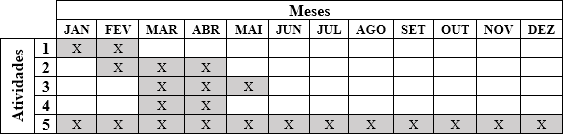
\includegraphics[scale=1]{imagens/cronograma}
\end{figure*}
\FloatBarrier

\begin{enumerate}
	\item Descrição da atividade 1;
	\item Descrição da atividade 2;
	\item Descrição da atividade 3;
	\item Descrição da atividade 4;
	\item Descrição da atividade 5.
\end{enumerate}
